\chapter{Idea and Requirements}
\label{chap:ideaAndRequirements}
\section{Product perspective}
A simple diagram of the common use of AlGa is here provided:
\begin{figure}[H]
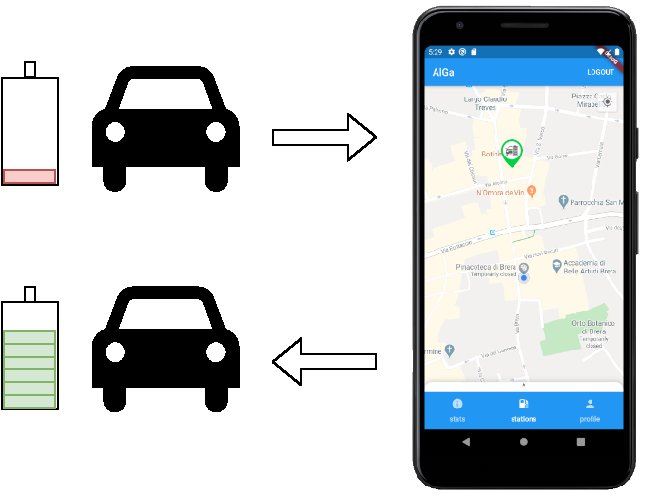
\includegraphics[width=\linewidth]{Pics/idea}
\caption{Use diagram of AlGa.}
\end{figure}
As we can see, AlGa is designed to help users directly on the road, in the fastest and easier way possible. Statistics useful for the users are another key part of the application: in fact, during the use, a set of useful metrics are collected and then displayed to the user. They can help her or him understand better the way in which they use their car, and fix some problems and/or wrong behaviors which may arise in the process of switching from a traditional car to an electric one. However, they are not strictly necessary to use the app; users can decide to opt-in to this functionality.
		
\section{Product functions}
According to the goals of the project, a more detailed description of the various functionalities is here provided:

\subsection*{Stations}
This is the default screen. It shows a map, centered on user's position, together with the charging stations. The user can select every station to see its properties like cost, position, vendor, etc (Requirement 1). If the user decides to utilize that station, a simple click on the ``GO'' button will open the Google Maps application, with the destination already defined on that station (Requirement 3).
Moreover, with a simple scroll menu, the user can also visualize a list of the nearest stations, with the possibility to order them by price, distance and speed and vendor (Requirement 2).

\subsection*{Stats}
The statistics screen provides the user with data about the use of their car and of the application. That is, the amount of time spent at charging stations, the amount of money spent in energy, the distance traveled and other aggregate information (Requirement 4). Leveraging the possibilities offered by sensors installed on every smartphone, AlGa can collect these statistics in an effortless way for the user.

\subsection*{Profile}
The profile screen lets the user customize their account on AlGa. They can choose a simple username, change their e-mail and password, and select their electric car. AlGa offers a list of cars from which the user can choose; every car has some statistics about the consumption, the autonomy etc. This leads to more accurate usage data (Requirement 5).

\section{User characteristics}
\begin{description}
\item[AlGa User:] An individual who has downloaded AlGa.
\item[Registered User:] An AlGa User who has created an account on AlGa platform.
\item[Vendor:] A company which offers electric recharging stations.
\end{description}

\section{Assumptions, dependencies and constraints}
\subsection*{Domain assumptions}
\begin{description}
    \item[{[D1]}] Users’ devices can provide precise and correct data on location.
    \item[{[D2]}] All cars are compatible with every recharge station.
    \item[{[D3]}] Cars' data inserted by users are correct.
\end{description}

\section{Performance Requirements}
AlGa can support a large amount of users, the only constraint is the plan of Firebase. 
The application, being designed in Flutter, can have native performances on Android devices. The goal is to support also older smartphones, given that no intensive operations are requested to devices' CPUs.

\section{Design Constraints}
\subsection{Standards compliance}
\begin{itemize}
    \item Permissions
    
	The app, in order to guarantee the use of AlGa, will request the following permissions (their name may vary between Android versions):
	\begin{itemize}
	    \item Geolocalization
	    \item Storage (if the user wants to upload a profile pic)
	\end{itemize}
    \item Other constraints
	\begin{itemize}
	    \item The app can be installed on SD card, if supported by Android version
	    \item AlGa is designed mainly for portrait use. Landscape mode is not officially supported.
	\end{itemize}
\end{itemize}

\subsection{Hardware limitations}
\begin{itemize}
    \item A smartphone with Android
    \item Internet connection
    \item GPS (optional)
\end{itemize}
		
\section{Software System Attributes}
\subsection{Reliability}
The reliability depends on the accuracy of charging stations' positions stored in Firebase. This responsibility is on the admins.

\subsection{Availability}
The service offered by AlGa has to be available 24/7. The system has to provide a proper way to avoid the possibility of denied service, i.e. to clone servers. This task is shifted on Firebase, which can be considered as a very reliable host.

\subsection{Security}
All the sensitive informations stored in the AlGa’s databases have to be stored securely in order to avoid any chance, for an external and not authorized user, to read the data. The sensitive information mentioned above are for all users the e-mail and the password. Also, the car and the recharge logs can be considered as a valuable data for an attacker.
On the servers, the security is guaranteed by Firebase policies, just admins can eventually access some data; passwords, however, are salted so neither admins can access them. 

